


%\documentclass[handout,xcolor=x11names,compress,10pt]{beamer}
\documentclass[xcolor=x11names,compress,10pt]{beamer}

\usepackage{../tslides} 
%% General document %%%%%%%%%%%%%%%%%%%%%%%%%%%%%%%%%%

\usepackage[romanian]{babel}

\setbeamertemplate{footline}[frame number]
\uselanguage{romanian}
\languagepath{romanian}

\deftranslation[to=romanian]{Proof}{Demonstra\c tie}
\deftranslation[to=romanian]{Example}{Exemplu}
\deftranslation[to=romanian]{Theorem}{Teorem\u a}
\deftranslation[to=romanian]{Solution}{Solu\c tie}
\deftranslation[to=romanian]{Lemma}{Lem\u a}
\deftranslation[to=romanian]{Definition}{Defini\c tie}

 

\lstset{language=Haskell}
\lstset{escapeinside={(*@}{@*)}}
\newcommand{\li}[1]{\lstinline$#1$}
 
%=========================================

\begin{document}
\title{\\Curs 4}
\author{Fundamentele Limbajelor de Programare} 
\date{2020-2021} 

\frame{\titlepage} 

%\frame{\frametitle{Cuprins}\tableofcontents} 

%\begin{frame}[fragile]{Monade cu structură de monoid}
%\vspace{-1ex}
%Definiția în biblioteca standard:
%\begin{asciihs}
%   class Monad m => MonadPlus m where
%     mzero :: m a
%     mplus :: m a -> m a -> m a
%
%   instance MonadPlus [] where
%      mzero     :: [a]
%      mzero     = []
%
%      mplus     :: [a] -> [a] -> [a]
%      mplus     = (++)
%
%   guard :: MonadPlus m => Bool -> m ()
%   guard False = mzero
%   guard True   = return ()
%
%   msum :: MonadPlus m => [m a] -> m a
%   msum = foldr mplus mzero
%\end{asciihs}
%\end{frame}


%Monads with plus
%In the standard prelude:

%\begin{frame}[fragile]{Descrieri de liste cu filtrare}
%\begin{asciihs}
%   pairs'' :: Int -> [(Int, Int)]
%   pairs'' n = [ (i,j) | i <- [1..n], j <- [1..n], i < j ]
%\end{asciihs}
%este echivalentă cu
%\begin{asciihs}
%   pairs''' :: Int -> [(Int, Int)]
%   pairs''' n = do {
%                    i <- [1..n];
%                    j <- [1..n];
%                    guard (i < j);
%                    return (i,j)
%                  }
%\end{asciihs}
%Exemplu
%\begin{asciihs}
%   *Main> pairs'' 4
%   [(1,2),(1,3),(1,4),(2,3),(2,4),(3,4)]
%   *Main> pairs''' 4
%   [(1,2),(1,3),(1,4),(2,3),(2,4),(3,4)]
%\end{asciihs}
%\end{frame}

\section{Analiză sintactică}\sectionframe

\begin{frame}[fragile]{Tipul unui analizor sintactic}
\begin{block}
{Prima încercare}
\begin{asciihs}
   type Parser a = String -> a
\end{asciihs}
\onslide<2->
\begin{itemize}
\item Dar cel puțin pentru rezultate parțiale, va mai rămâne ceva de analizat
\end{itemize}
\end{block}
%
%Second attempt:
\onslide<3->
\begin{block}
{A doua încercare}
\begin{asciihs}
   type Parser a = String -> (a, String)
\end{asciihs}
\onslide<4>
\begin{itemize}
\item Dar dacă gramatica e ambiguă?
\item Dar dacă intrarea nu corespunde nici unui element din a?
\end{itemize}
\end{block}
\end{frame}


%Parser type
%
%
%
%                         A parser for things
%                     is a function from strings
%                           to lists of pairs
%                        Of things and strings
%                                             —Graham Hutton
\begin{frame}[fragile]{Tipul unui analizor sintactic}{A treia încercare}
\hfill \href{http://www.willamette.edu/~fruehr/haskell/seuss.html}{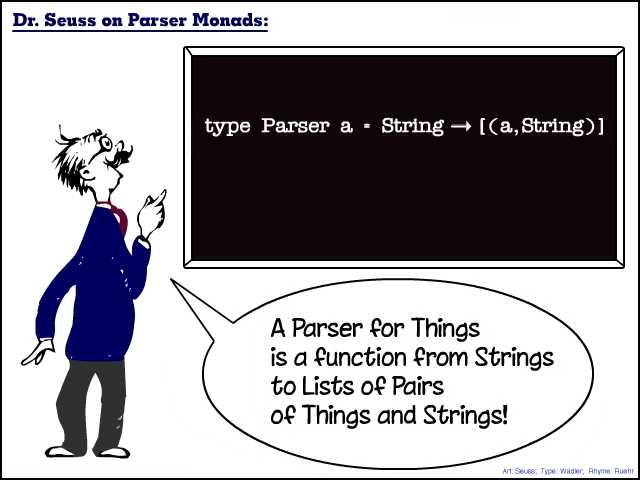
\includegraphics[scale=.4]{SeussFinal2}}\hfill\;
\end{frame}

\begin{frame}[fragile]{Tipul Parser}

\begin{block}{Tipul Parser}
\begin{asciihs}
  
  newtype Parser a =
    Parser { apply :: String -> [(a, String)] }
\end{asciihs}
\end{block}

\begin{asciihs}
  -- Folosirea unui parser 
  -- apply :: Parser a -> String -> [(a, String)]
  -- apply (Parser f) s = f s

  -- Daca exista parsare, da prima varianta
  parse :: Parser a -> String -> a
  parse m s = head [ x | (x,t) <- apply m s, t == "" ]
\end{asciihs}
\end{frame}


%Module Parser




%Parser is a Monad




%Parser is a Monad with Plus
%  -- Some monads have additional structure
%

\begin{frame}[fragile]{Parsare pentru caractere}
\begin{asciihs}
  -- Recunoasterea unui caracter
  anychar :: Parser Char
  anychar = Parser f
    where
    f []     = []
    f (c:s) = [(c,s)]
\end{asciihs}
\pause

\begin{asciihs}
*Main> parse anychar "a"
'a'
*Main> parse anychar "ab"
*** Exception: Prelude.head: empty list

*Main> apply anychar "abc"
[('a',"bc")]
\end{asciihs}
\end{frame}

\begin{frame}[fragile]{Parsare pentru caractere}
\begin{asciihs}
 -- Recunoasterea unui caracter cu o proprietate
  satisfy :: (Char -> Bool) -> Parser Char
  satisfy p = Parser f
    where
    f []                 = []
    f (c:s) | p c        = [(c, s)]
            | otherwise = []
\end{asciihs}
\pause 
\begin{asciihs}
*Main> parse (satisfy isUpper) "A"
'A'
(0.01 secs, 52,760 bytes)
*Main> parse (satisfy isUpper) "a"
*** Exception: Prelude.head: empty list

*Main> apply (satisfy isUpper) "Ab"
[('A',"b")]
\end{asciihs}
\end{frame}


\begin{frame}[fragile]{Parsare pentru caractere}
\begin{asciihs}
  -- Recunoasterea unui anumit caracter
  char :: Char -> Parser Char
  char c = satisfy (== c)
\end{asciihs}

\pause 
\begin{asciihs}
*Main> parse (char 'a') "a"
'a'
(0.00 secs, 52,824 bytes)
*Main> parse (char 'a') "ab"
*** Exception: Prelude.head: empty list

*Main>  apply (char 'a') "ab"
[('a',"b")]
\end{asciihs}
\end{frame}

\begin{frame}[fragile]{Parsarea unui cuvânt cheie}
\begin{asciihs}
-- Recunoasterea unui cuvant cheie
string :: String -> Parser String
string [] = Parser (\s -> [([],s)])
string (x:xs) = Parser f  
 where
   f s = [(y:z,zs)| (y,ys) <- apply (char x) s, 
                    (z,zs) <- apply (string xs) ys]
\end{asciihs}

\pause
\begin{asciihs}
*Main> parse (string "abc") "abc"
"abc"
*Main> parse (string "abc") "abcd"
*** Exception: Prelude.head: empty list

"*Main> apply  (string "abc") "abcd"
[("abc","d")]
\end{asciihs}
\end{frame}
%Parsing characters

\begin{frame}[fragile]{Monada Parser}
\begin{asciihs}

  --   class Monad m where
  --     return :: a -> m a
  --     (>>=) :: m a -> (a -> m b) -> m b

  instance Monad Parser where
    return x  = Parser (\s -> [ (x, s) ])
    m >>= k   = Parser (\s -> [ (y, u)
                              | (x, t) <- apply m s
                              , (y, u) <- apply (k x) t
                              ])
\end{asciihs}
\end{frame}

\begin{frame}[fragile]{Monada Parser}
\begin{asciihs}
-- Recunoasterea unui cuvant cheie
string :: String -> Parser String
string [] = Parser (\s -> [([],s)])
string (x:xs) = Parser f  
 where
   f s = [(y:z,zs)| (y,ys) <- apply (char x) s, 
                    (z,zs) <- apply (string xs) ys]
\end{asciihs}

e echivalent cu 

\begin{asciihs}
  string :: String -> Parser String
  string []     = return []
  string (x:xs) = do  y  <- char x
                      ys <- string xs
                      return (y:ys)

\end{asciihs}
\end{frame}


\begin{frame}[fragile]{Combinarea variantelor}
\begin{asciihs}

digit = satisfy isDigit
abcP = satisfy (`elem` ['A','B','C'])

alt :: Parser a -> Parser a -> Parser a
alt p1 p2 = Parser f
          where f s = apply p1 s ++ apply p2 s 
\end{asciihs}

\pause 
\begin{asciihs}
*Main> apply (alt digit abcP) "1sd"
[('1',"sd")]
*Main> apply (alt digit abcP) "Asd"
[('A',"sd")]
*Main> apply (alt digit abcP) "dsd"
[] 
*Main> parse (alt digit abcP) "A"
'A'
*Main> parse (alt digit abcP) "1"
'1'
\end{asciihs}
\end{frame}

\begin{frame}[fragile]{ Parser e monadă cu plus}
\begin{asciihs}
  --   class MonadPlus m where
  --     mzero :: m a
  --     mplus :: m a -> m a -> m a

  instance MonadPlus Parser where
    mzero      = Parser (\s -> [])
    mplus m n  = Parser (\s -> apply m s ++ apply n s)
               -- === alt m n
\end{asciihs}

\begin{itemize}
\item mzero reprezintă analizorul sintactic care eșuează tot timpul
\item mplus reprezintă combinarea alternativelor
\end{itemize}


\begin{asciihs}
instance Alternative Parser where
  empty  = mzero
  (<|>) = mplus  
\end{asciihs}
\end{frame}


\begin{frame}[fragile]{ Parser e monadă cu plus}
\begin{asciihs}
instance MonadPlus Parser where
    mzero      = Parser (\s -> [])
    mplus m n  = Parser (\s -> apply m s ++ apply n s)

instance Alternative Parser where
  empty  = mzero
  (<|>) = mplus  
\end{asciihs}

\begin{asciihs}
*Main> apply (digit <|> abcP) "1www"
[('1',"www")]
*Main> apply (digit <|> abcP) "Awww"
[('A',"www")]
*Main> parse (digit <|> abcP) "B"
'B'
*Main> parse (digit <|> abcP) "2"
'2'
\end{asciihs}
\end{frame}


\begin{frame}[fragile]{Recunoașterea unui caracter cu o proprietate}
\begin{block}{Alternative și Gărzi}
\begin{asciihs}
guard :: MonadPlus f => Bool -> f ()
guard True = return ()
guard False = mzero
\end{asciihs}
\end{block}
\begin{asciihs}
  satisfy :: (Char -> Bool) -> Parser Char
  satisfy p = Parser f
    where
    f []                 = []
    f (c:s) | p c        = [(c, s)]
            | otherwise = []
\end{asciihs}
e echivalentă cu
\begin{asciihs}
  satisfy :: (Char -> Bool) -> Parser Char
  satisfy p = do   c <- anychar
                   guard (p c)
                   return c
\end{asciihs}

\end{frame}
%Parsing a string

\begin{frame}[fragile]{Recunoașterea unei secvențe repetitive}
\begin{asciihs}
  -- Steluta Kleene (zero, una sau mai multe repetitii)
  many :: Parser a -> Parser [a]
  many p  =  some p   `mplus`   return []

  -- cel putin o repetitie
  some :: Parser a -> Parser [a]
  some p = do   x <- p
                xs <- many p
                return (x:xs)
\end{asciihs}
\end{frame}


%Parsing a sequence

\begin{frame}[fragile]{Recunoașterea unui numar întreg}
\begin{asciihs}
  -- Recunoasterea unui numar natural
  decimal :: Parser Int
  decimal = do  s <- some digit
                return (read s)

  -- Recunoasterea unui numar negativ
  negative :: Parser Int
  negative = do   char '-'
                  n <- decimal
                  return (-n)

  -- Recunoasterea unui numar intreg
  integer :: Parser Int
  integer = decimal `mplus` parseNeg
\end{asciihs}
\end{frame}


%Parsing an integer


\begin{frame}[fragile]{Recunoașterea unui identificator}

\begin{block}{Cum arată un identificator}
  Un identificator este definit de doi parametri

  \begin{itemize}
    \item felul primului caracter (e.g., începe cu o literă)
    \item felul restului caracterelor (e.g., literă sau cifră)
  \end{itemize}
\end{block}

Dat fiind un parser pentru felul primului caracter și un parser pentru
felul următoarelor caractere putem parsa un identificator:

\begin{asciihs}
  -- Recunoasterea unui identificator
  identifier :: Parser Char -> Parser Char -> Parser String
  identifier firstCh nextCh = do   c <- firstCh
                                   s <- many nextCh
                                   return (c : s)
\end{asciihs}

Exemplu
\begin{asciihs}
  myId = identifier (satisfy isAlpha) (satisfy isAlphaNum)
\end{asciihs}
\end{frame}



\begin{frame}[fragile]{Eliminarea spațiilor}

\begin{block}{Ignorarea spațiilor}
\begin{asciihs}
skipSpace :: Parser ()
skipSpace = do  _ <- many (satisfy isSpace)
                return ()
\end{asciihs}
\end{block}


\begin{block}{Ignorarea spațiilor de dinainte și după}
\begin{asciihs}
token :: Parser a -> Parser a
token p = do  skipSpace
              x <- p
              skipSpace
              return x
\end{asciihs}
\end{block}

\end{frame}
  
  

\begin{frame}[fragile]{Modulul Exp}
\begin{asciihs}
  module Exp where

  import Monad
  import Parser

  data Exp = Lit Int
           | Exp :+: Exp
           | Exp :*: Exp
           deriving (Eq,Show)

  evalExp   :: Exp -> Int
  evalExp   (Lit n)    = n
  evalExp   (e :+: f) = evalExp e + evalExp f
  evalExp   (e :*: f) = evalExp e * evalExp f
\end{asciihs}
\end{frame}


%Module Exp


\begin{frame}[fragile]{Recunoașterea unei expresii}
\begin{asciihs}
  parseExp :: Parser Exp
  parseExp = parseLit `mplus` parseAdd `mplus` parseMul
    where
    parseLit = do   n <- integer
                    return (Lit n)
    parseAdd = do   char '('
                    d <- token parseExp
                    char '+'
                    e <- token parseExp
                    char ')'
                    return (d :+: e)
    parseMul = do   char '('
                    d <- token parseExp
                    char '*'
                    e <- token parseExp
                    char ')'
                    return (d :*: e)
\end{asciihs}
\end{frame}


%Parsing an expression

\begin{frame}[fragile]{Recunoașterea și evaluarea unei expresii}{Test}
\begin{asciihs}
  *Exp> parse parseExp "(1 + (2 * 3))"
  Lit 1 :+: (Lit 2 :*: Lit 3)
  *Exp> evalExp (parse parseExp "(1 + (2 * 3))")
  7
  *Exp> parse parseExp "( ( 1 + 2 ) * 3 )"
  (Lit 1 :+: Lit 2) :*: Lit 3
  *Exp> evalExp (parse parseExp "( ( 1 + 2 ) * 3 )")
  9
\end{asciihs}
\end{frame}

\begin{frame}{}
\vfill\begin{center}
\intens{Pe s\u apt\u am\^ana viitoare!}
\end{center}
\vfill
\end{frame}

\end{document}



